\documentclass[a4paper,12pt]{article}
\usepackage[brazil]{babel}
\usepackage[utf8]{inputenc}
\usepackage{amsmath,amssymb}
\usepackage[a4paper,margin=0.8in]{geometry}
\usepackage{tikz}
\usetikzlibrary{patterns}



\begin{document}

\title{Quizz 1 e 2 - Search e Knwoledge}
\author{BCC325 - Intelligência Artificial}
\date{}
\maketitle


\section*{Search}

\begin{enumerate}
\item Entre busca em profundidade (DFS - Depth First Search) e busca em largura (BFS - Breadth First Search), qual encontrará um caminho mais curto através de um labirinto? Justifique a sua resposta.

\begin{enumerate}
    \item DFS sempre encontrará um caminho mais curto do que BFS
    \item BFS sempre encontrará um caminho mais curto do que DFS
    \item DFS às vezes, mas nem sempre, encontrará um caminho mais curto do que BFS
    \item BFS às vezes, mas nem sempre, encontrará um caminho mais curto do que DFS
    \item Ambos os algoritmos sempre encontrarão caminhos do mesmo comprimento
\end{enumerate}


\item Considere o labirinto abaixo. Células cinzas indicam paredes. Um algoritmo de busca foi executado neste labirinto e encontrou o caminho destacado em amarelo, que vai do ponto A ao ponto B. No processo, as células destacadas em vermelho foram os estados explorados que não levaram ao objetivo.

\begin{figure}[!ht]
    \centering
    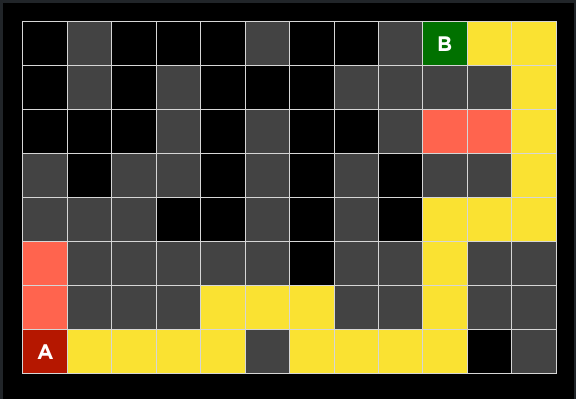
\includegraphics[scale=0.5]{maze.png}
\end{figure}

Dos quatro algoritmos de busca discutidos na aula — busca em profundidade, busca em largura, busca gulosa com heurística de distância de Manhattan e busca A* com heurística de distância de Manhattan — qual deles (ou quais, se for o caso) poderia ser o algoritmo utilizado? Justifique a sua resposta.

\begin{enumerate}
    \item Poderia ser apenas A*
    \item Poderia ser apenas a busca gulosa
    \item Poderia ser apenas DFS
    \item Poderia ser apenas BFS
    \item Poderia ser A* ou a busca gulosa
    \item Poderia ser DFS ou BFS
    \item Poderia ser qualquer um dos quatro algoritmos
    \item Não poderia ser nenhum dos quatro algoritmos
\end{enumerate}


\item Por que o minimax com profundidade limitada às vezes é preferível ao minimax sem limite de profundidade?

\begin{enumerate}
    \item O minimax com profundidade limitada pode chegar a uma decisão mais rapidamente porque explora menos estados
    \item O minimax com profundidade limitada produzirá o mesmo resultado que o minimax sem limite de profundidade, mas pode, às vezes, usar menos memória
    \item O minimax com profundidade limitada pode tomar uma decisão mais ótima ao não explorar estados sabidamente subótimos
    \item O minimax com profundidade limitada nunca é preferível ao minimax sem limite de profundidade
\end{enumerate}

\item Considere a árvore Minimax abaixo, onde as setas verdes para cima indicam o jogador MAX e as setas vermelhas para baixo indicam o jogador MIN. Os nós folha estão rotulados com seus respectivos valores.
Qual é o valor do nó raiz?


\begin{figure}[!ht]
    \centering
    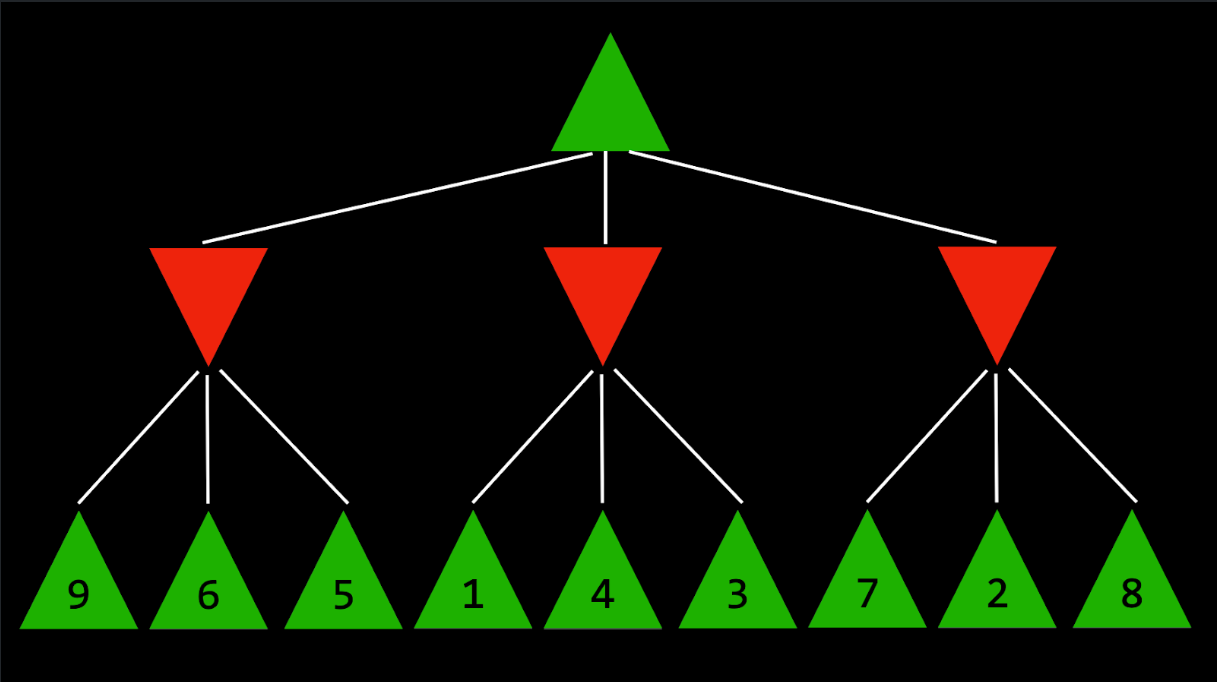
\includegraphics[scale=0.3]{min_max.png}
\end{figure}


\item Considere o seu arquivo \textit{degrees.py}. Qual linha de código determina o tipo de algoritmo de busca que você implementou? Justifique a sua respposta. 

\item Considere o seu arquivo \textit{tictactoe.py}. Neste código, quem é o max player, isto é, o jogador que tenta maximizar o retorno do jogo? 

\end{enumerate}

\section*{Knowledge}

\begin{enumerate}
\item Considere as seguintes sentenças lógicas:

\begin{itemize}
    \item 1 - Se Hermione está na biblioteca, então Harry está na biblioteca.
    \item 2 - Hermione está na biblioteca.
    \item 3 - Ron está na biblioteca e Ron não está na biblioteca.
    \item 4 - Harry está na biblioteca.
    \item 5 - Harry não está na biblioteca ou Hermione está na biblioteca.
    \item 6 - Ron está na biblioteca ou Hermione está na biblioteca.
\end{itemize}

Qual das seguintes implicações lógicas é verdadeira?

\begin{enumerate}
    \item A Sentença 6 implica a Sentença 2
    \item A Sentença 1 implica a Sentença 4
    \item A Sentença 6 implica a Sentença 3
    \item A Sentença 2 implica a Sentença 5
    \item A Sentença 1 implica a Sentença 2
    \item A Sentença 5 implica a Sentença 6
\end{enumerate}

\item Existem outros conectivos lógicos além dos discutidos na aula. Um dos mais comuns é o "OU Exclusivo" (representado pelo símbolo $\oplus$). A expressão $A \oplus B$ representa a sentença "A ou B, mas não ambos." Qual das seguintes é logicamente equivalente a $A \oplus B$?

\begin{enumerate}
    \item $(A \lor B) \land \neg (A \land B)$
    \item $(A \land B) \lor \neg (A \lor B)$
    \item $(A \lor B) \land (A \land B)$
    \item $(A \lor B) \land \neg (A \lor B)$
\end{enumerate}

\item Seja a variável proposicional $R$ "Está chovendo," a variável $C$ "Está nublado," e a variável $S$ "Está ensolarado." Qual das seguintes é uma representação lógica proposicional da sentença "Se está chovendo, então está nublado e não está ensolarado."?

\begin{enumerate}
    \item $(R \to C) \land \neg S$
    \item $R \to C \to \neg S$
    \item $R \land C \land \neg S$
    \item $R \to (C \land \neg S)$
    \item $(C \lor \neg S) \to R$
\end{enumerate}

\item  Considere, na lógica de primeira ordem, os seguintes predicados. $Student(x)$ representa o predicado "x é um estudante." $Course(x)$ representa o predicado "x é um curso." $Enrolled(x, y)$ representa o predicado "x está matriculado em y." Qual das seguintes é uma tradução em lógica de primeira ordem da sentença "Existe um curso no qual Harry e Hermione estão ambos matriculados."?

\begin{enumerate}
    \item $\exists x.\ Course(x) \land Enrolled(Harry, x) \land Enrolled(Hermione, x)$
    \item $\forall x.\ Course(x) \land Enrolled(Harry, x) \land Enrolled(Hermione, x)$
    \item $\exists x.\ Enrolled(Harry, x) \land \exists y.\ Enrolled(Hermione, y)$
    \item $\forall x.\ Enrolled(Harry, x) \land \forall y.\ Enrolled(Hermione, y)$
    \item $\exists x.\ Enrolled(Harry, x) \lor Enrolled(Hermione, x)$
    \item $\forall x.\ Enrolled(Harry, x) \lor Enrolled(Hermione, x)$
\end{enumerate}

\item Considere o puzzle 1 no seu código em \textit{puzzle.py}. Como você modelou a informação de que um Trapaceiro (Knave) mente?

\item Considere o se código em \textit{minesweeper.py}. Explique a função \texttt{mark\_safe}

\end{enumerate}

\end{document}
